\documentclass[12pt,titlepage]{report}


\usepackage[italian]{babel} %italiano
\usepackage[T1]{fontenc} 
\usepackage[utf8]{inputenc}
\usepackage{graphicx} %immagini
\usepackage{hyperref}
\usepackage{fancyhdr}
\usepackage[nouppercase]{frontespizio}

\pagestyle{fancy}

\renewcommand{\chaptermark}[1]%
{\markboth{\MakeUppercase{\thechapter.\ #1}}{}}
\renewcommand{\sectionmark}[1]%
{\markright{\MakeUppercase{\thesection.\ #1}}}
\renewcommand{\headrulewidth}{0.5pt}
\renewcommand{\footrulewidth}{0pt}
\newcommand{\helv}{%
\fontfamily{phv}\fontseries{b}\fontsize{9}{11}\selectfont}
\fancyhf{}
\fancyhead[LE,RO]{\helv \thepage}
\fancyhead[LO]{\helv \rightmark}
\fancyhead[RE]{\helv \leftmark}


\graphicspath{ {./img/} }
\linespread{1.23}

% Copyright 2017 Sergei Tikhomirov, MIT License
% https://github.com/s-tikhomirov/solidity-latex-highlighting/

\usepackage{listings, xcolor}

\definecolor{verylightgray}{rgb}{.97,.97,.97}

\lstdefinelanguage{Solidity}{
	keywords=[1]{anonymous, assembly, assert, balance, break, call, callcode, case, catch, class, constant, continue, constructor, contract, debugger, default, delegatecall, delete, do, else, emit, event, experimental, export, external, false, finally, for, function, gas, if, implements, import, in, indexed, instanceof, interface, internal, is, length, library, log0, log1, log2, log3, log4, memory, modifier, new, payable, pragma, private, protected, public, pure, push, require, return, returns, revert, selfdestruct, send, solidity, storage, struct, suicide, super, switch, then, this, throw, transfer, true, try, typeof, using, value, view, while, with, addmod, ecrecover, keccak256, mulmod, ripemd160, sha256, sha3}, % generic keywords including crypto operations
	keywordstyle=[1]\color{blue}\bfseries,
	keywords=[2]{address, bool, byte, bytes, bytes1, bytes2, bytes3, bytes4, bytes5, bytes6, bytes7, bytes8, bytes9, bytes10, bytes11, bytes12, bytes13, bytes14, bytes15, bytes16, bytes17, bytes18, bytes19, bytes20, bytes21, bytes22, bytes23, bytes24, bytes25, bytes26, bytes27, bytes28, bytes29, bytes30, bytes31, bytes32, enum, int, int8, int16, int24, int32, int40, int48, int56, int64, int72, int80, int88, int96, int104, int112, int120, int128, int136, int144, int152, int160, int168, int176, int184, int192, int200, int208, int216, int224, int232, int240, int248, int256, mapping, string, uint, uint8, uint16, uint24, uint32, uint40, uint48, uint56, uint64, uint72, uint80, uint88, uint96, uint104, uint112, uint120, uint128, uint136, uint144, uint152, uint160, uint168, uint176, uint184, uint192, uint200, uint208, uint216, uint224, uint232, uint240, uint248, uint256, var, void, ether, finney, szabo, wei, days, hours, minutes, seconds, weeks, years},	% types; money and time units
	keywordstyle=[2]\color{teal}\bfseries,
	keywords=[3]{block, blockhash, coinbase, difficulty, gaslimit, number, timestamp, msg, data, gas, sender, sig, value, now, tx, gasprice, origin},	% environment variables
	keywordstyle=[3]\color{violet}\bfseries,
	identifierstyle=\color{black},
	sensitive=false,
	comment=[l]{//},
	morecomment=[s]{/*}{*/},
	commentstyle=\color{gray}\ttfamily,
	stringstyle=\color{red}\ttfamily,
	morestring=[b]',
	morestring=[b]"
}

\lstset{
	language=Solidity,
	backgroundcolor=\color{verylightgray},
	extendedchars=true,
	basicstyle=\footnotesize\ttfamily,
	showstringspaces=false,
	showspaces=false,
	numbers=left,
	numberstyle=\footnotesize,
	numbersep=9pt,
	tabsize=2,
	breaklines=true,
	showtabs=false,
	captionpos=b
}
 %solidity color
%\begin{lstlisting}[language=Solidity]
%\end{lstlisting}

\begin{document}

\begin{frontespizio}
\Universita{Torino}
\Facolta{Scieze della Natura}
\Corso[Laurea]{Informatica}
\Logo[7.5cm]{./img/Unito-logo}
\Titoletto{Tesi di laurea}
\Titolo{Studio e realizzazione di un prototipo di un sistema basato su blockchain per il mobility as a service}
\Candidato[880847]{Giorgio Mecca}
\Relatore{Prof.~Claudio Schifanella}
\Annoaccademico{2020-2021}
\end{frontespizio}

%\author{Giorgio Mecca}
%\title{Studio e realizzazione di un prototipo di un sistema basato su blockchain per il mobility as a service}
%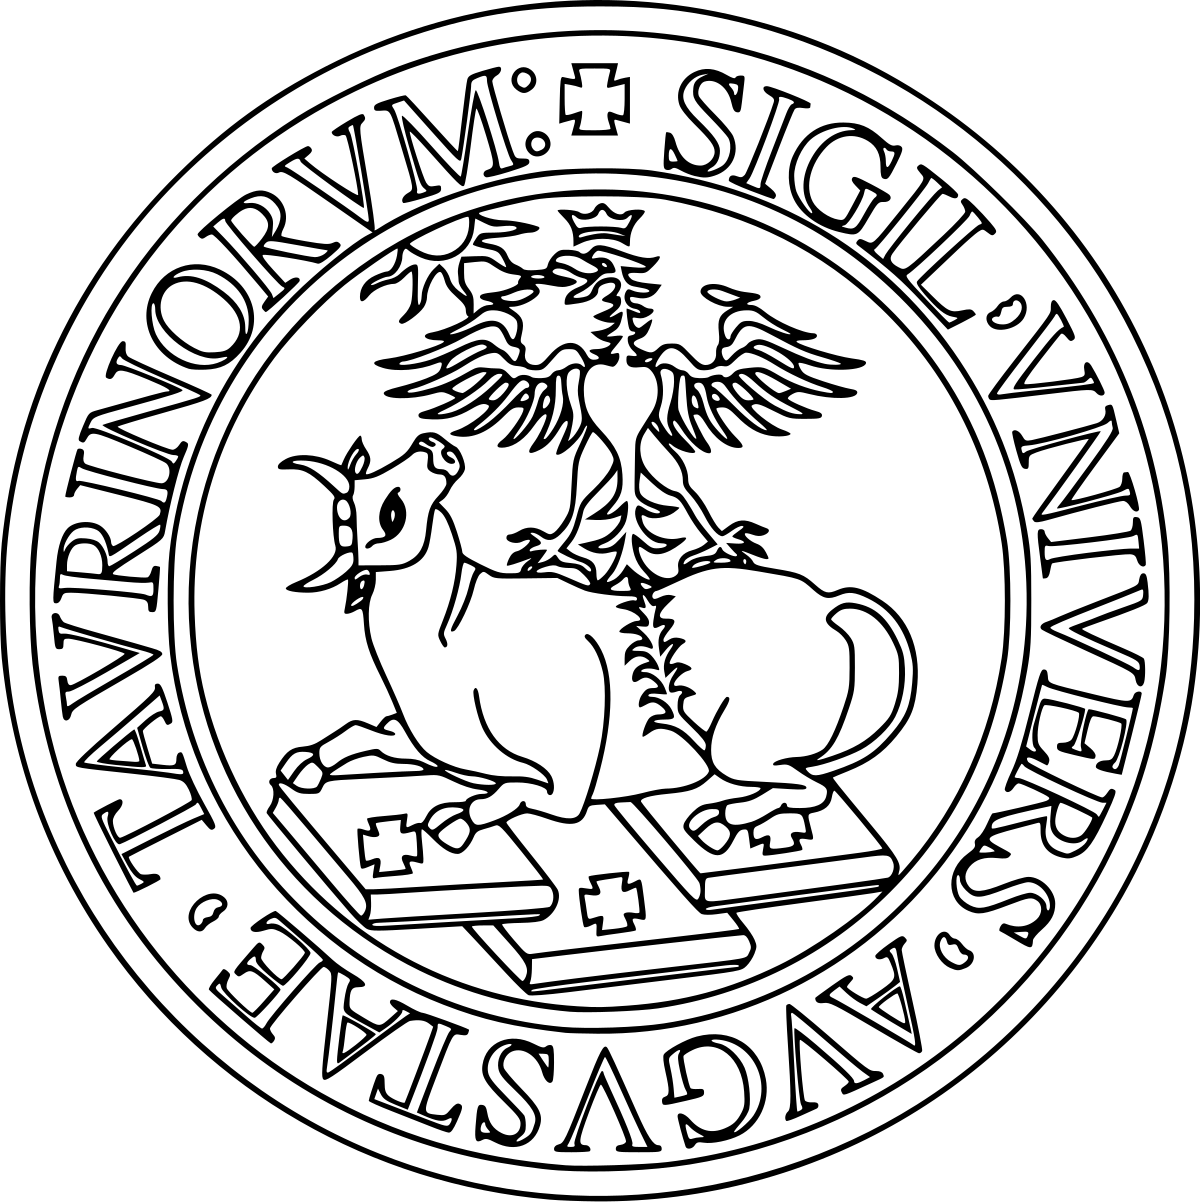
\includegraphics[height=.2\textheight]{Unito-logo}
%\maketitle
%Study and realization of a prototype of a blockchain-based system for mobility as a service

%abstract
\begin{abstract} 
Il seguente elaborato descrive lo studio effettuato sulla tecnologia blockchain durante il tirocinio presso la 2+consulting. Lo studio è stato svolto ponendo particolare attenzione sulle blockchain private, la differenza e i vantaggi con le tecnologie pubbliche. In seguito ho dedicato la mia concentrazione allo studio di come e se fosse possibile avviare una blockchain privata scegliendo come tecnologia il client Besu, client facente parte del gruppo Hyperlegder che utilizza la tecnologia Etherium. Una volta definiti e studiati i parametri di essa, come ad esempio il meccanismo del consenso da utilizzare scegliendo IBFT 2.0 basato su PoA, ho studiato il modello di gestione e utilizzo di blockchain con gli Smart Contract, che permettono inoltre di inserire e memorizzare dati su blockchain includendo dati sulle transazioni pubbliche da certificare. In questo modo si è svolto uno studio sui dati utilizzati e come gestire il modello di Blockchain Ibrida, cioè l'utilizzo concatenato di una blockchain privata utilizzata per le sue proprietà sulla sicurezza e quindi come ente certificatore decentralizzato e un DataBase relazionale così da poter interrogare e accedere con facilità ai dati. Il passo finale è stato sviluppare una Web app con tipologia Single Page Application utilizzando come server la tecnologia Node Js con l'utilizzo del framework Web3 per l'interfacciamento alla blockchain. La Web app è sviluppata con l'ideologia della possibile integrazione nel Mobility as Service. Questa caratteristica è stata sviluppata con l'ideologia di fornire ai vari enti partecipanti un diverso account(coppia di chiavi pubblica e privata) che si utilizzerà per l'interfacciamento e gli fornirà determinati accessi. La WebApp ha quindi permesso la distinzione dei vari utenti che, in base al loro ruolo, avranno accessi e possibilità diverse sull'app. Queste possibilità riguardano chi e quali dati dovrà inserire e chi invece può interrogare le informazioni a cui ha accesso.
\end{abstract}

%indice
\tableofcontents

%capitolo 1
\chapter{Introduzione}
\section{Descrizione del Progetto}
\section{Descrizione dell’azienda}

%capitolo 2
\chapter{Blockchain}
\section{Problema dei generali bizantini}
\begin{figure}[h]
	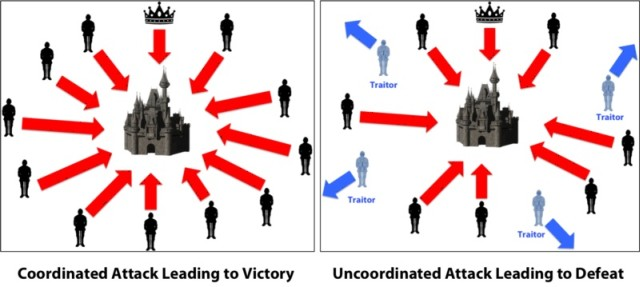
\includegraphics[width=\textwidth]{BF}
	\centering
	\caption{Problema dei generali bizantini}
	\label{fig:ByzantinFault}
\end{figure}

Il problema dei generali bizantini è un problema informatico su come raggiungere il consenso in situazioni in cui è possibile la presenza di errori. Il problema consiste nel trovare un accordo, comunicando solo tramite messaggi, tra componenti diversi nel caso in cui siano presenti informazioni discordanti. Il problema è stato teorizzato dai matematici Leslie Lamport, Marshall Pease e Robert Shostak nel 1982, i quali crearono la metafora dei generali, caso di studio molto utilizzato nei sistemi basati o che comunque utilizzano una network. La metafora si basa su diversi generali che durante un assedio sono sul punto di attaccare una città nemica. Essi sono dislocati in diverse aree strategiche e possono comunicare solo mediante messaggeri al fine di coordinare l'attacco decisivo (Figura \ref{fig:ByzantinFault}). I generali possono attaccare o ritirarsi, l'importante e che ci sia una decisione unanime, l'utilizzo di sola metà forza bellica porterebbe ad una sconfitta o una perdita. Il problema risiede quindi nell'alta probabilità che tra questi vi sia un generale traditore che mandi messaggi che vanno contro la strategia dell'esercito. La possibile soluzione punta al trovare un meccanismo secondo il quale un generale non traditore che riceva più messaggi sappia riconoscere quello veritiero. Secondo l'articolo di Lamport, Shostak e Pease non esiste una soluzione se il numero di processi non corretti è maggiore o uguale a un terzo del numero totale di processi. Una soluzione proposta è quella di Nakamoto che in una sua stesura sulla blockchain descrive un meccanisco per arrivare al consenso chiamato PoW Proof of Work.

\section{Struttura di una blockchain}
\begin{figure}[h]
	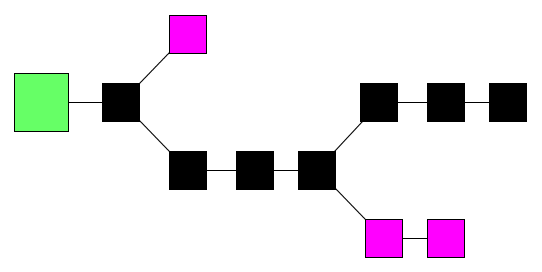
\includegraphics[width=\textwidth]{bl1}
	\centering
	\caption{Rappresentazione struttura di una blockchain}
	\label{fig:blockchain1}
\end{figure}

Una Blockchain come suggerisce l'etimologia della parola è una catena di blocchi o DLT - Distributed Ledger Technology. È una struttura dati formata da un insieme di blocchi(struttura prioritaria) collegati univocamente 1 ad 1 così da creare una metaforica catena. Una blockchain è considerata una struttura condivisa e immutabile in quanto il suo contenuto una volta scritto non è più né modificabile né eliminabile, a meno di non invalidare l'intera struttura. Questa tecnologia fà parte dei Distributed Legder cioè dei "libri mastro distribuiti" o registri condivisi infatti tutti i partecipanti della blockchain, detti anche nodi, posseggono lo stesso registro cioè le stesse informazioni andando a costruire il contrapposto di una struttura centralizzata come un Database, quindi una struttura Decentralizzata in cui ogni nodo ha la possibilità di leggere autonomamente le informazioni contenute.
Nella figura \ref{fig:blockchain1} viene visualizzata una semplice blockchain in cui sono presenti tre tipologie di blocchi quali, il blocco verde visto come il blocco di genesi, i blocchi neri che vanno a costituire la catena principale e i blocchi viola considerati blocchi orfani. L'aggiunta di un nuovo blocco è globalmente regolata da un protocollo condiviso e se autorizzata ogni nodo aggiorna la propria copia privata del registro così da evitare manipolazioni future. In una blockchain i nodi partecipanti vengono anche chiamati minatori- miner o validatori, riferendosi al loro compito nella rete rispetto ai blocchi.

\section{Hashing}
Un codice hash è una qualunque sequenza di caratteri alfanumerici generati da una particolare funzione di hash. Questa funzione prende in input un qualunque tipo di informazione e restituisce una stringa di lunghezza prefissata, questo rende la funzione one-way o non invertibile in quanto conoscendo il digest(codice hash restituito) non è possibile risalire all'informazione che lo ha generato. In una blockchain l'Hash viene utilizzato per la costruzione della catena, viene calcolato l'hash di un blocco e il blocco che lo succederà avrà come parametro questo hash. In questo modo ogni blocco è legato univocamente al blocco precedente e siccome il codice hash di un blocco viene calcolato utilizzando anche il codice hash precedente modificando un singolo blocco verrà invalidata tutta la struttura blockchain immediatamente successiva.
\begin{figure}[h]
	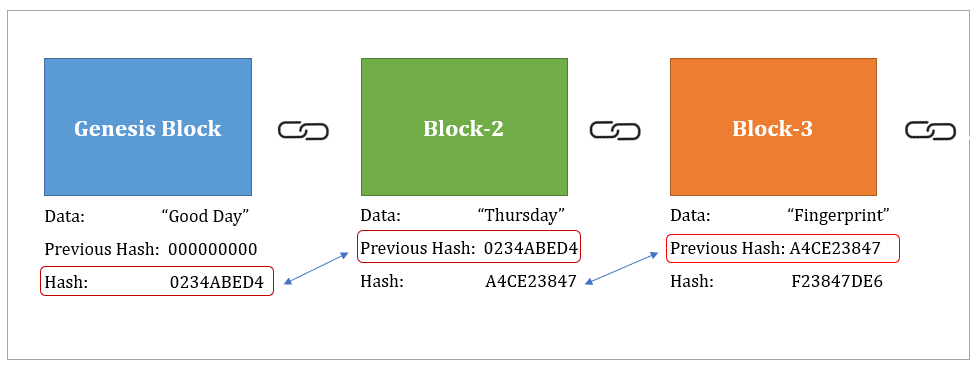
\includegraphics[width=\textwidth]{bc1}
	\centering
	\caption{Catena di una blockchain}
	\label{fig:blockchain2}
\end{figure}

\section{Transazioni}
\begin{figure}[h]
	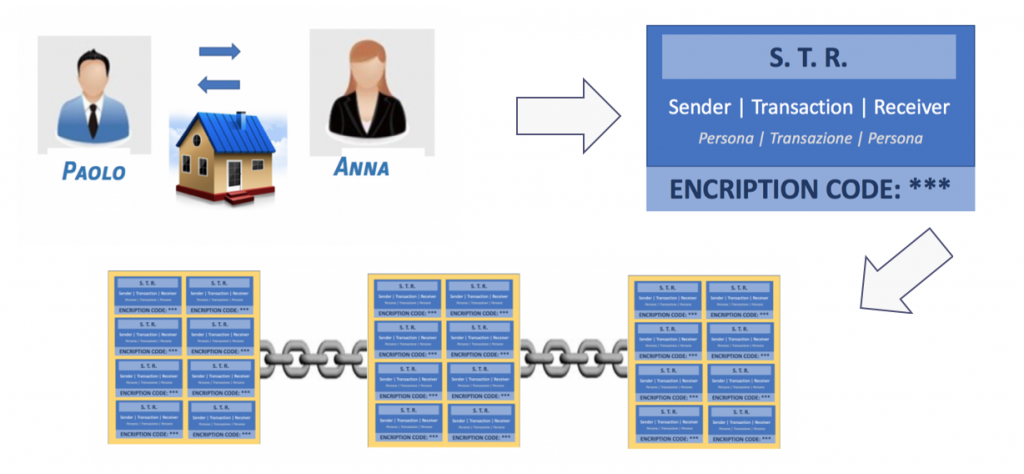
\includegraphics[width=\textwidth]{flusso_bc}
	\centering
	\caption{Flusso di esecuzione di una Transazione}
	\label{fig:fl_bc}
\end{figure}
In una blockchain i dati vengono scritti sotto forma di Transazioni in seguito contenute in vari blocchi. L'uso più comune delle transazioni è l'invio di denaro o in qualche modo una moneta equivalente. Le transazioni devono quindi avere un mittente, un destinatario, un 'value' cioè il valore trasmesso, vengono quindi considerate come un cambio di stato riferendosi alle informazioni nella blockchain e saranno identificate da un Transaction Hash. Una volta inviata, la transazione entra in un transaction pool, da dove i miner andranno a selezionare randomicamente transazioni da includere nel prossimo blocco. Una transazione per essere considerata valida deve essere accettata da un nodo che la inserirà nel blocco che sta minando, non è certo che due nodi che minano lo stesso blocco la inseriscano nella stessa posizione.

\section{Blocchi}
La blockchain è una sequanza di blocchi che contengono una collezione di Transazioni.  il numero di transazioni all'interno di ognuno di questi blocchi varia in base alla dimensione della transazione stessa.I blocchi sono prodotti dai nodi validators e vengono generati in un lasso di tempo definito dalle regole della blockchain(Es: 15 secondi per Ethereum, 10 min per BitCoin), nel momento in cui il blocco viene completato i dati contenuti diventano verificati.

\begin{figure}[h]
	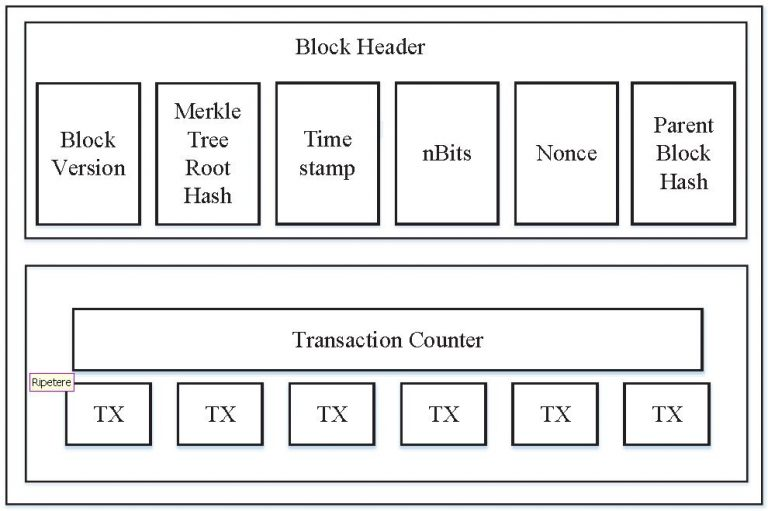
\includegraphics[width=\textwidth]{bcbl}
	\centering
	\caption{Struttura di un Blocco}
	\label{fig:blockblockchain1}
\end{figure}

Un Blolcco è diviso in due parti, l`header e il body. Le transazioni sono racchiuse nel body del blocco e nell'header sono presenti i campi di gestione del blocco stesso come descritto nella figura \ref{fig:blockblockchain1}.


\begin{itemize}
  \item Versione del blocco: indica le regole di validazione del blocco da rispettare
  \item Merkle Tree Root Hash valore della radice del Merkle Tree in cui sono salvate le transazioni del blocco
  \item TimeStamp: Marca temporale salvata come Timestamp UNIX che indica l`inserimento del blocco nella blockchain
  \item nBits: è la soglia target di un hash di blocco valido
  \item Nonce: è un campo il cui valore è settato dai miner così che l’hash del blocco
calcolato sia minore o uguale al target attuale della rete(difficoltà). Dato che non
è possibile prevedere la combinazione di bit che risulterebbero nell’hash voluto,
numerosi valori di nonce sono calcolati fino a quando l’hash risultante rispetti i
requisiti attuali della rete.
\item Parent Block Hash: segna l'hash del blocco a cui verrà agganciato
\end{itemize}

Il Body è composto da un contatore di transazioni (transaction counter) e dalle transazioni (TX), queste vengono memorizzate e organizzate tramite un Merkle Tree cioè una struttura ad albero in cui le foglie contengono i digest hash delle informazioni mentre i nodi contengono i digest hash dei nodi sottostanti(figli)
\begin{figure}[h]
	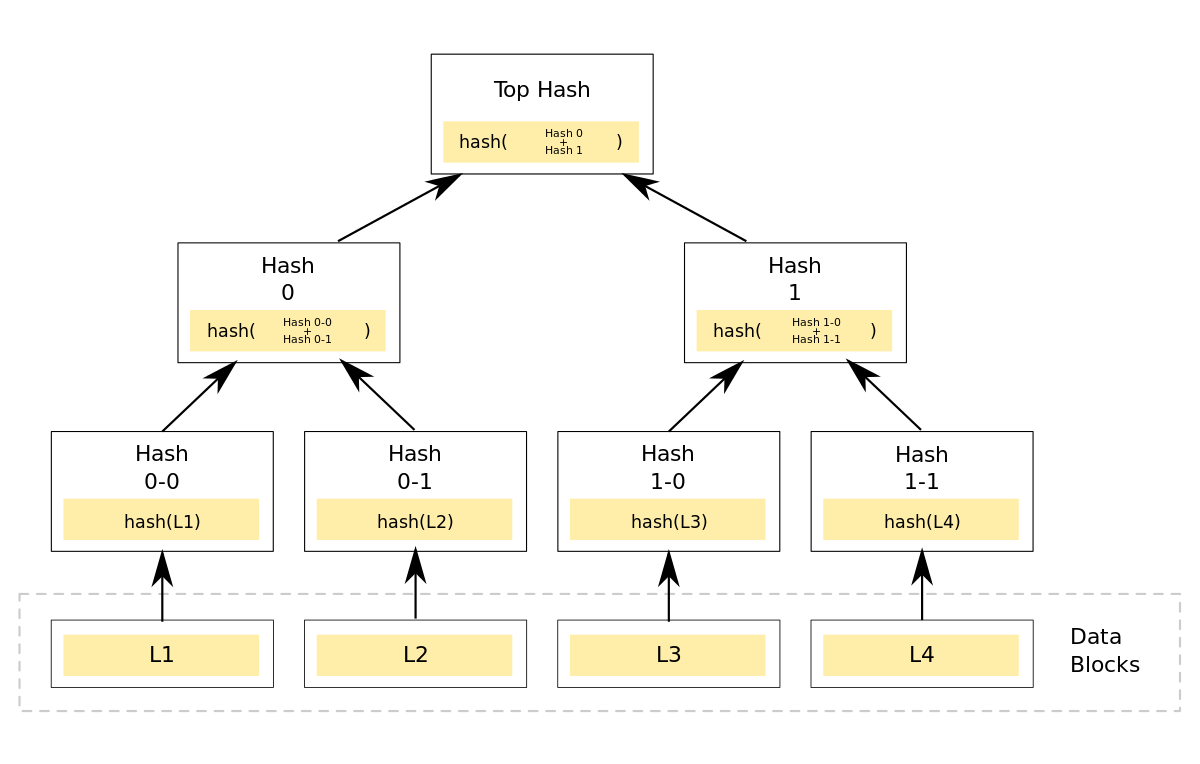
\includegraphics[width=\textwidth]{Hash_Tree}
	\centering
	\caption{Merkle Tree}
	\label{fig:Tree1}
\end{figure}

\section{Mining e Meccanismi del consenso}
I miner sono i nodi partecipanti alla rete che  ascoltano le transazioni inviate, verificano che non siano malevole e compongono un blocco organizzando le transazioni in un Merkle Tree.
I minatori che 'calcolano' un blocco valido vengono premiati con un incentivo (Es: criptovaluta)
È anche possibile che più miner producano lo stesso blocco e la scelta del blocco da seguire per la catena spetta al meccanismo del consenso cioè  il set di regole che permette la finalizzazione delle transazioni e il funzionamento del sistema così che tutti i nodi della rete convergano ad una sola versione condivisa della catena, questo andrà a creare una biforcazione o Fork da cui si avranno una sequenza valida(quella che verrà continuata) e una sequenza(anche un singolo nodo) orfana(Figura \ref{fig:blockchain1}).

\subsection{Consenso Trustless}
La blockhain è considerata Trustless, letteralmente "senza fiducia" poiché a differenza di un sistema centralizzando non esiste nessun ente centrale in cui riporre la fiducia(come ad esempio una Banca,governi o istituti finanziari). Utilizzando un sistema decentralizzato la fiducia non viene eliminata definitivamente ma viene suddivisa tra tutti i partecipanti, in questo modo più sarà alto il numero dei partecipanti meno fiducia si dovrà affidare ad ogni singolo nodo. La fiducia viene quindi riposta nei singoli nodi e che questi rispettino le regole considerate valide.

\subsection{Proof of Work}
L'algoritmo del consenso più famoso ed utilizzato(come da Bitcoin, Ethereum e Monero) nonché il primo algoritmo del consenso mai creato è il PROOF OF WORK abbreviato PoW. Questo si basa sulla "Prova del Lavoro" svolto dai miner che dovranno risolvere unauna serie di operazioni considerate u puzzle matematico per poter creare un blocco valido. Il primo miner che costruisce il blocco lo aggiunge alla catena, notifica in broadcast il resto della rete e di conseguenza tutte le transazioni in esso presenti vengono validate, infine il miner viene ricompensato con un incentivo come una moneta che sarà relativa quello che gli utenti pagano per effettuare le transazioni, cioè le "tasse" - fees. I miner quindi utilizzano la loro potenza e le risorse computazionali per provare che hanno svolto del lavoro(questo produce anche un massivo consumo di elettricità), talvolta è possibile che due o più nodi producano lo stesso blocco creando un fork e quindi due differenti catene. Il sistema è incentivato a scrivere nuovi blocchi sulla catena più lunga così da eliminare la biforcazione orfana e ricondurre tutta la rete a un`unica catena, questo implica che se si voglia creare un blocco "falso" e farlo accettare dalla blockchain bisognerà possedere una potenza di calcolo maggiore di tutta la rete. Il mining diventa sempre più competitivo con la partecipazione di sempre più gente e con l'aumentare della difficoltà, perciò si è vista la creazione delle Mining Pool cioè un insieme di persone che raggruppa la propria potenza di calcolo per il mining di criptomoneta, in questo modo la probabilità di costruire un blocco valido aumenta e di conseguenza aumenta anche il guadagno suddiviso tra i partecipanti

\subsection{Proof of Stake}
\begin{figure}[h]
	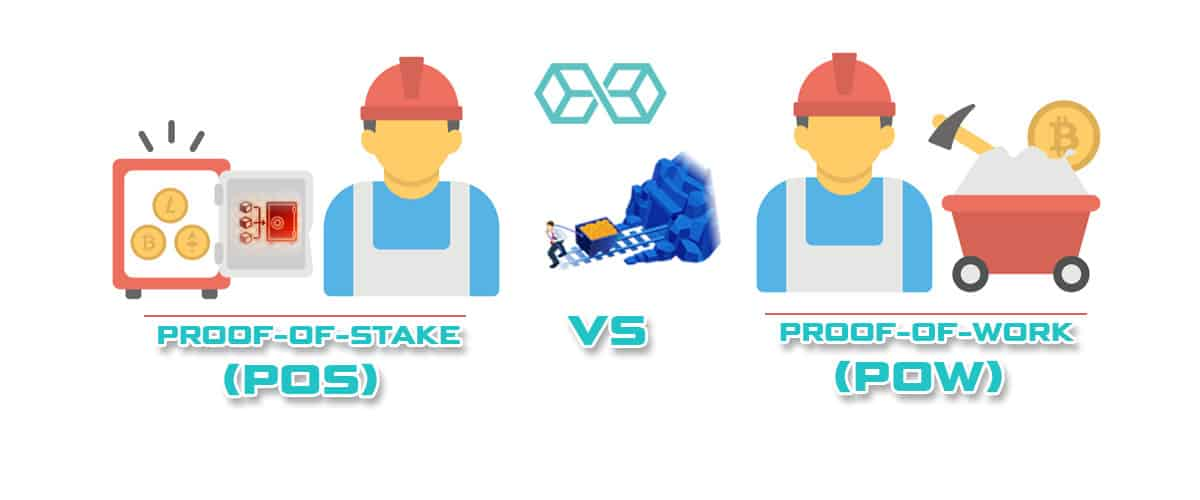
\includegraphics[width=\textwidth]{pow-pos}
	\centering
	\caption{PoW-PoS}
	\label{fig:pow-pos}
\end{figure}

Nel 2011 basandoci sui problemi del PoW come il dispendio di energia elettrica o la creazione di grosse Mining Pool che elimina la decentralizzazione si è sviluppata l`idea del PoS Proof of Stake. Il PoS sostituisce i miner con i validatori o coniatore, questi per far si che il loro blocco venga considerato valido devono depositare della moneta come "cauzione" che viene appunto chiamata Stake. 
In questo modo se con il PoW era possibile inserire transazione fraudolente qui si andrebbe a perdere la somma congelata. Il criterio di scelta dei validatori si basa sulla quantità di moneta bloccata la durata del blocco, con il secondo parametro si va in contro al problema generato dal primo parametro cioè che solo i più ricchi possono essere scelti e quindi diventare più ricchi.
L’elezione del blocco leader (da aggiungere) avviene tramite l’algoritmo VFR – Verifiable random function che utilizza l’algoritmo “follow-the-coin” - “più denaro blocchi più hai fiducia”. Il PoS porta molteplici vantaggi rispetto al PoW come un minimo dispendio energetico e una maggiore sicurezza e decentralizzazione dovuta all`assenza di mining pool.

\subsection{Proof of Authority}
\begin{figure}[h]
	
\includegraphics[height=.4\textheight]{judge}
\end{figure}
Un ultimo algoritmo del consenso è il PoA - Proof of Autority. Qui viene meno il concetto di decentralizzazione in quanto si basa sull'utilizzo di nodi validatori noti. Il PoA viene spesso utilizzato in ambito privato o militare e si utilizza, come intuibile dal nome, il concetto di Autorità che quindi avrà il potere di decidere i nodi validatori, cioè gli unici nodi che potranno produrre blocchi, mentre gli altri nodi avranno soltanto la possibilità di lettura. Il PoA fa si che i nodi validatori mettano in "Stake" la loro reputazione a differenza di una moneta. Il modello Proof of Authority consente alle imprese di mantenere la propria privacy e allo stesso tempo avvalersi dei vantaggi della tecnologia blockchain. Inoltre il modello PoA riduce il problema del consumo in quanto diventa inutilizzabile il concetto di concorrenza nel mining e di conseguenza le mining pool. Riferendosi al Trilemma della scalabilità PoA rinuncia alla decentralizzazione a favore della sicurezza.

\section{Attacchi}
Nonostante la blockchain sta avendo molteplici riscontri positivi negli ultimi anni la sua caratteristica di decentralizzazione la rende si più affidabile rispetto ad un sistema centralizzato ma risultano comunque possibili e attuabili degli Attacchi ad essa.

\subsection{Selfish Mining Attack}
\begin{figure}[h]
	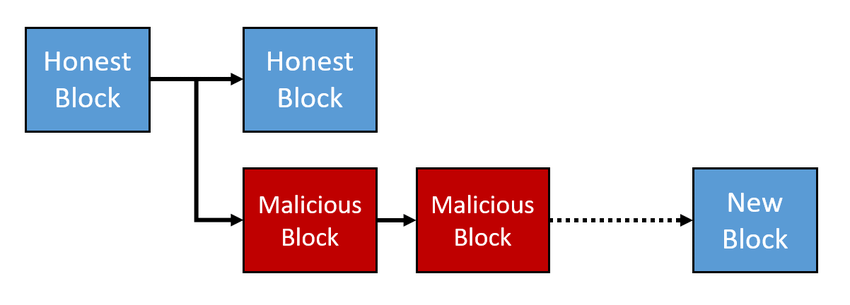
\includegraphics[width=\textwidth]{Selfish-mining-attack}
	\centering
	\caption{Selfish-mining-attack}
	\label{fig:SM-attack}
\end{figure}
Il Selfish Mining Attack si basa su un sistema PoW e sfrutta la sua debolezza nel momento in cui si genera un Fork. Nel momento in cui si genera una biforcazione solo la catena più lunga viene considerata valida e le transazioni nella catena orfana vengono rese nulle. Per l`attuarsi del Selfish Mining Attack si ha bisogno che l`attaccante cioè il Faul-Miner generi un blocco che potrebbe creare un Fork (in cui si ha la possibilità di inserire transazioni fraudolente) ma lo tenga segreto, senza aggiungerlo alla Blockchain. Il Fault-Miner dovrà continuare a generare blocchi seguendo la sua catena e quando questa sarà più lunga di quella che attualmente gli altri miner stanno seguendo, pubblicherà il suo Fork e la sua catena che essendo più lunga secondo l`algoritmo del PoW verrà considerata valida e sarà quella che gli altri miner seguiranno da quel momento in poi. Per l`attuazione del Selfish Mining Attack si ha bisogno quindi che un singolo ente possegga più del 51% della potenza dell`intera rete.

\subsection{Double Spending Attack}
\begin{figure}[h]
	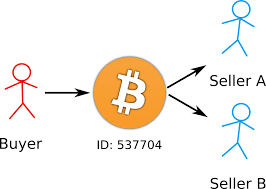
\includegraphics[height=0.2\textheight]{dsa}
	\centering
	\caption{Double Spending Attack}
	\label{fig:ds-attack}
\end{figure}
Il Double Spending Attack viene concepito per la possibilita di spedere due volte la stessa moneta. Questo potrebbe essere attuabile con la creazione di due diverse transazioni. Le due transazioni però dovranno appartenere a due blocchi diversi, e se due miner che competono nel minare un blocco utilizzano ognuno una transazione diversa? Allora verranno prodotti due blocchi con entrambe le transazioni MA verrà prodotto un Fork quindi sono una delle due transazioni verrà poi validata mentre la seconda sarà annullata, ricordando che una transazione o meglio un blocco ha una validità pari al numero di blocchi minati in seguito (In BitCoin un blocco è validato se sono stati prodotti 6 blocchi successivi).

\section{Blockchain Pubbliche/Private}
Una blockchain pubblica solitamente è anche detta permissionless, letteralmente "senza permessi" cioè un nuovo nodo non ha bisogno di speciali permessi per partecipare quindi minare o effettuare transazioni nella rete che quindi viene definita pubblica. Le reti permissionless sono quindi decentralizzate in quanto nessuno ha il controllo della rete.

Le blockchain private sono conosciute come permissioned, sono caratterizzate dalla presenza di un’autorità centrale che decide chi può accedere e assegna loro un ruolo nella rete che determinerà cosa il nuovo nodo avrà il permesso di fare, se ha la possibilità di partecipare alla rete o se potrà essere un nodo validatore o sola lettura . La sicurezza di una blockchain privata fa maggiormente perno sull'affidabilità dei singoli partecipanti.

\section{Ethereum}

\begin{figure}[h]
	
\includegraphics[height=0.2\textheight]{eth}
	\centering
	\caption{Etherium Logo}
	\label{fig:eth-logo}
\end{figure}

Ethereum è una piattaforma decentralizzata ideata nel 2013 (in seguito pubblicata nel 2015) come sostituto a BitCoin. Ethereum è una piattaforma basata su blockchain che permette quindi la gestione degli smart contract e come Bitcoin mette a disposizione una moneta che viene analogamente chiamata Ether e abbreviata con ETH. La moneta viene utilizzata per le varie transazioni ma viene anche usata per pagare le "tasse" - fee, nello specifico viene utilizzato un sottomultiplo dell'ETH chiamato wei che corrisponde a circa  $ 10^{-18} $ ETH  ( 1 ETH = $ 10^{18} $ wei). Per lo sviluppo e interfacciamento viene messa a disposizione da Ethereum la EVM - Ethereum Virtual Machine che funge da macchina turing completa in grado di eseguire byte code. La sua funzione è quella di consentire l'esecuzione di programmi o smart contract al fine di implementare una serie di funzionalità aggiuntive su detta blockchain; la Evm utilizza per gli smart contract un linguaggio di alto livello specializzato chiamato Solidity.

\subsection{Smart Contract}
\subsection{Solidity}
\subsection{Gas}

Quando si effettua una transazione o si carica uno smart contract la VM richiede un pagamento calcolato in gas. Il gas è una frazione dell'ether e viene richiesto per un'operazione come l'invio di una transazione infatti viene comunemente chiamato "transaction fee". Il gas viene anche richiesto quando si effettua una qualunque operazione tramite uno smart contract e dipende dala complessità di essa.
\subsection{Dapps}

%capitolo 3
\chapter{Tecnologie utilizzate}
\section{Besu}
\subsection{IBFT}
\subsubsection{IBFT Methods}
\subsection{Free Gas Network}
\subsection{API Methods}
\section{Truffle}
\subsection{Compile}
\subsection{Test}
\subsection{Deploy}
\section{Node js}
\subsection{Web3}

%capitolo 4
\chapter{Caso d'uso}
\section{Problema Iniziale}
Il progetto blockchain è stato ideato e sviluppato come proposta di soluzione ai problemi nella gestione del tracciamento, invio, certificazione e mantenimento di dati riguardanti "spostamenti". Questi spostamenti sono informazioni(LOG) inviate da un qualunque ente che metta a disposizione della società o di un qualunque servizio che preveda dei mezzi pubblici o privati quali ad esempio autobus, treni, taxi etc... Queste informazioni vengono ora raccolte, analizzate e utilizzate su di modelli di storage a fogli di calcolo (Ad Esempio EXCEL - Programma Micrsoft). I fogli di calcolo offrono alcuni vantaggi come la semplicità con cui vengo creati, scritti e salvati benché offrano un'interfaccia poco user friendly('facilmente utilizzabile') guardando tutti i possibili attori, mentre il progetto si focalizza sui difetti come la pubblicazione/condivisione delle informazioni o l'interrogazione di queste in quanto utilizzando semplici fogli non vengono proposte alcune regole di struttura e organizzazione,e ci si pone particolare importanza alla sicurezza e all'affidabilità di queste informazioni e che non vengano modificate durante la condivisione, quindi la possibile certificazione di essi.

\section{Soluzione}
La soluzione proposta si offre di risolvere tutti i problemi sopra elencati come la certificazione, salvataggio e interrogazioni di informazioni. Viene ideata una blockchain privata che avrà funzione di ente (decentralizzato) certificatore, questa non utilizza nessuna moneta creando una Free Gas Network e che con l'ausilio di appositi smart contract(scritti e caricati autonomamente) ci permette di salvare un codice che andrà ad identificare un determinato gruppo di spostamenti come un codice Hash che usufruendo della struttura e utilizzo della blockchain non potrà essere modificato, ciò implica che si potrà sempre verificare la correttezza del gruppo di spostamenti richiesti ricreando e controllando il loro codice.

La memorizzazione dei dati viene invece affidata ad un database relazionale, utilizzando nel progetto il DBMS(DataBase Managenent System) MySql, che ci permette di salvare grandi quantità di dati con una efficiente organizzazione gestita con la creazione di tabelle così da essere facilmente interrogabile in futuro.
 
L'interfaccia comune è gestita con un server sviluppato tramite tecnologia node js che con una single Page Application avrà la funzione di interfaccia user friendy con funzioni di memorizzazione per i log degli spostamenti su Database, calcolo e salvataggio dei loro codici hash sulla blockchain al tempo stimato e quando necessario, cioè quando e ovunque verranno richiesti dei dati e avverrà l'interrogazione del DataBase sarà reso obbligatorio il controllo di questi con il codice sulla blockchain. Inserendo questo WebServer intermedio o server proxy si andrà ad eliminare il passaggio di dati non propriamente protetto e rende partecipi tutti i singoli attori dell'attività.

\subsection{Problematiche}
Utilizzando delle nuove tecnologie sorgono comunque nuove problematiche che non sono state affrontate nello sviluppo in quanto non inerenti ai fini del progetto.

%DOS utilizzando un solo server
Una prima problematica si sviluppa utilizzano un server proxy. Avendo un singolo server di accesso al database a alla blockchain sequesto non viene correttamente protetto e costantemente controllato è soggetto ai classici attacchi come un DDOS - Distributed Denial of Service in cui si utilizzano molteplici messaggi fittizi (come un inizio di HandShake per una connessione TCP) per far si che il server non possa sostenere tutti i servizi e essendo l'unico punto di accesso bloccherebbe  l'intero accesso alla rete blockchain.

%blockchain utile solo con molti nodi
Una caratteristica che rende sicura la blockchain pubblica è la molteplicità di nodi, questa con una blockchain privata come la nostra va a decadere con il discendere  del numero di nodi; utilizzando un meccanisco di conseso basato su PoA(Proof of Autority) si ha infatti bisogno di un minimo di 4 nodi per essere resistente al problema bizantino.

%attacco del compleanno
Per evitare l'appesantimento della Blockchain si è pensato di salvare su di essa solo un codice identificativo(codice Hash) per un gruppo di Log. Questo implica che con l'aumentare dei log identificati da un singolo codice hash diminuisca la sicurezza che questo apporta infatti sarà più facilmente utilizzabile un attacco come l'attacco del compleanno che ha come obiettivo quello di generare una collisione cioè di trovare dei dati fittizi ai Log originari che però generano lo stesso codice Hash, questi dati fittizi potranno essere quindi sostituiti nel DB ma verranno comunque considerati certificati dal sistema in quanto produrranno lo stesso codice.

\section{Attori}
Il caso d'uso per il progetto blockchain prevede la partecipazione di diversi attori quali: 

Un Terminal User o utente finale è un comune dipendente di un ente che partecipa alla blockchain il quale ha il compito di comunicare i propri spostamenti/Log o qualunque informazione di cui si preveda il salvataggio;

Gli Admin sono dei dipendenti di enti partecipanti che vengono segnati dagli stessi come amministratori che quindi posseggono  particolari oneri come il possesso e la trasmissione di una chiave privata;

Il proprietario/gestore della blockchain avrà il compito di gestire l'intera blockchain privata con l'amministrazione che ne segue, come la supervisione dei nodi presenti, il loro funzionamento e la loro caratterizzazione come validatori. 
\section{Scenario di utilizzo}
Il Progetto prevede uno scenario di utilizzo diverso seguendo la distinzione degli attori.
Per l'utilizzo si prevede che ad ogni ente partecipante al progetto gli venga assegnato un account, cioè una copia di chiavi privata e pubblica che serviranno per interagire con la blockchain, inoltre ogni ente dovrà inserire i propri dipendenti nel Database e specificare il ruolo di essi, se admin o Terminal User.

Un Terminal User, una volta effettuato l'accesso, viene portato ad un'interfaccia in cui può inserire la città che sarà selezionata come Start dello spostamento e in seguito viene spostato in una seconda interfaccia da cui può terminare lo spostamento o annullarlo, se annullato potrà cominciare un nuovo spostamento dalla precedente interfaccia, il completamento di questo avverrà solo se compila i campi necessari quali la città di Termine e la distanza percorsa indicata in Kilometri.

Un admin, una volta effettuato l'accesso, potrà a differenza di un Terminal User effettuare delle query/ interrogazioni riguardo gli spostamenti compiuti, inserendo una data otterrà tutti gli spostamenti che sono stati certificati da una transazione inserita in quella determinata data, da qui potrà anche accedere ai dettagli della transazione o del blocco che la contiene riferendoci alla blockchain, inoltre, quando il sistema lo richiede, ha il compito di inserire la Private Key dell'utente(ente) che verrà utilizzata per la scrittura su blockchain.

%capitolo 5
\chapter{Sviluppo}
\section{Schema Progetto}
\section{Blockchain Ibrida}
\section{Smart Contract}
\subsection{Boxing}
\section{WebApp}
\subsection{Single Page Application}
\subsection{Input}
\subsubsection{Inserimento in un DB}
\subsubsection{Inserimento nella Blockchain}
\subsection{Output}
\subsubsection{Report di Controllo}
\subsubsection{Monitor Blockchain}

%capitolo 6
\chapter{Sviluppi futuri}
\section{Analisi costi}
\section{Immissione nella blockchain pubblica}
\section{Blockchain pubblica come certificazione}
\section{Svilupo full Blockchain}


%lista delle Immagini
\listoffigures

\end{document}
